\documentclass[hidelinks,12pt]{article}
\usepackage[utf8]{inputenc}
\usepackage[table,xcdraw]{xcolor}
\usepackage{mathtools}
\usepackage{amsthm}
\usepackage{amsmath}
\usepackage{amsfonts}
\usepackage{amssymb}
\usepackage{centernot}
\usepackage{marvosym}
\usepackage{enumitem}
\usepackage{hyperref}
\usepackage{graphicx}
\graphicspath{{/home/theo/Documents/GitHub/Math-Homeworks/Math 531/Random/}}
\setcounter{tocdepth}{1}
\let\marvosymLightning\Lightning
\newtheorem{theorem}{Theorem}
\newtheorem{corollary}{Corollary}[theorem]
\newtheorem*{remark}{Remark}
\renewcommand\qedsymbol{QED}
\newcommand{\C}{\mathbb{C}}
\newcommand{\R}{\mathbb{R}}
\newcommand{\N}{\mathbb{N}}
\newcommand{\Z}{\mathbb{Z}}
\newcommand{\Q}{\mathbb{Q}}
\newcommand{\divby}{%
  \mathrel{\text{\vbox{\baselineskip.65ex\lineskiplimit0pt\hbox{.}\hbox{.}\hbox{.}}}}%
  }
\newcommand{\notdivby}{\centernot\divby}
\title{\scalebox{2}{Math 531 Exam 1}}
\author{\scalebox{1.5}{Theo Koss}}
\date{March 2021}
\begin{document}
\begin{titlepage} % Suppresses displaying the page number on the title page and the subsequent page counts as page 1
	\newcommand{\HRule}{\rule{\linewidth}{0.5mm}} % Defines a new command for horizontal lines, change thickness here
	
	\center % Centre everything on the page
	
	%------------------------------------------------
	%	Headings
	%------------------------------------------------
	
	\textsc{\LARGE University of Wisconsin-Milwaukee}\\[1.5cm] % Main heading such as the name of your university/college
	
	\textsc{\Large Modern Algebra}\\[0.5cm] % Major heading such as course name
	
	\textsc{\large Math 531}\\[0.5cm] % Minor heading such as course title
	
	%------------------------------------------------
	%	Title
	%------------------------------------------------
	
	\HRule\\[0.4cm]
	
	{\huge\bfseries Exam 2}\\[0.4cm] % Title of your document
	
	\HRule\\[1.5cm]
	
	%------------------------------------------------
	%	Author(s)
	%------------------------------------------------
	
	\begin{minipage}{0.4\textwidth}
		\begin{flushleft}
			\large
			\textit{Author}\\
			Theodore \textsc{Koss} % Your name
		\end{flushleft}
	\end{minipage}
	~
	\begin{minipage}{0.4\textwidth}
		\begin{flushright}
			\large
			\textit{Supervisor}\\
			Dr. Burns \textsc{Healy} % Supervisor's name
		\end{flushright}
	\end{minipage}
	
	% If you don't want a supervisor, uncomment the two lines below and comment the code above
	%{\large\textit{Author}}\\
	%John \textsc{Smith} % Your name
	
	%------------------------------------------------
	%	Date
	%------------------------------------------------
	
	\vfill\vfill\vfill % Position the date 3/4 down the remaining page
	
	{\large\today} % Date, change the \today to a set date if you want to be precise
	
	%------------------------------------------------
	%	Logo
	%------------------------------------------------
	
	%\vfill\vfill
	%\includegraphics[width=0.2\textwidth]{placeholder.jpg}\\[1cm] % Include a department/university logo - this will require the graphicx package
	 
	%----------------------------------------------------------------------------------------
	
	\vfill % Push the date up 1/4 of the remaining page
	
\end{titlepage}
\section{Problem 1}Let $n$ be an integer greater than 1.  For the symmetric group on $n$ letters, find a normal subgroup. Describe the quotient of $S_n$ by this normal subgroup.\begin{proof}For all groups $S_n$ where $n>1\in \Z$, the alternating group, $A_n=\{\sigma\in S_n|\sigma\text{ is even}\}$. This is a subgroup by the (aptly named) Subgroup Test \begin{theorem}[Subgroup Test]\label{sgtest}Let $G$ be a group and let $H$ be a nonempty subset of $G$. If for all $a,b\in H$, $ab^{-1}\in H$, then $H\leqslant G$. \end{theorem}Proof of \ref{sgtest} \href{https://en.wikipedia.org/wiki/Subgroup_test}{\color{cyan}here}\newline Suppose $\mu,\sigma\in A_n$, then $\mu=\tau_1\dots \tau_{2k}$ and $\sigma=\tau'_1\dots\tau'_{2m}$. $\sigma^{-1}=\tau'_{2m}\dots\tau'_1$. Then  $\mu\sigma^{-1}=\underbrace{\tau_1\dots \tau_{2k}\tau'_{2m}\dots\tau'_1}_{2(k+m)\text{ transpositions}}$. And since $2(k+m)$ is even, $\mu\sigma^{-1}\in A_n$ and thus $A_n$ is a subgroup.\newline $|A_n|=\frac{n!}{2}$ by \href{https://en.wikipedia.org/wiki/Alternating_group}{\color{cyan}{This}} result in math. Thus, since $|S_n|=n!$, $S_n-A_n=\{\sigma\in S_n|\sigma\text{ is odd}\}$, these two sets, $A_n$ and $S_n-A_n$ describe the quotient of $S_n$.
\end{proof}
\section{Problem 2}Let $G=Z\oplus Z$ be the group determined by pairs of integers, where addition is defined by adding each component. Find three (proper, not the whole group) subgroups of $G$ none of which are isomorphic to each other. Prove that one of these subgroups is isomorphic to $G$ itself, and is normal. Describe the quotient group of $G$ by this last group.\begin{proof} 3 Subgroups:
\begin{enumerate}[label=(\arabic*)]
    \item $H=\{(x,0)|x\in G\}$. By the subgroup test, if $\forall a,b\in H,\quad ab^{-1}\in H$ then it is a subgroup. $ab^{-1}=(a-b,0)$, and since $a-b\in G$  this is a subgroup.
    \item $H'=\{(0,y)|y\in G\}$. By the subgroup test, if $\forall a,b\in H,\quad ab^{-1}\in H$ then it is a subgroup. $ab^{-1}=(0,a-b)$, and since $a-b\in G$  this is a subgroup.
    \item $F=\{(x,y)|x,y\in2\Z\}$. By the subgroup test, if $\forall a,b\in H,\quad ab^{-1}\in H$ then it is a subgroup. $ab^{-1}=(x_1-x_2,y_1-y_2)$, and since even integer minus another even integer is always an even integer, both $(x_1-x_2)\in 2\Z$ and $(y_1-y_2)\in 2\Z$.\newline Conjecture: $G\approxeq F$. Let $\phi:G\to F$ be a function which takes $a=(x,y)\in G$ to $a'=(2x,2y)\in F$, defined by $\phi(a)=2a=a'\in F$. (It just doubles the input from $G$) N2S:. \begin{enumerate}[label=\roman*]
        \item $\phi:G\to F$ is a homomorphism.\newline Consider some elements $a,b\in G$, such that $\phi(a)=a'\in F$ and $\phi(b)=b'\in F$. $$\phi(a+b)=a'+b'=\phi(a)+\phi(b)$$
        \item $\phi:G\to F$ is injective. \newline $\forall a\in G$ $\exists a'\in F$ such that $\phi(a)=a'$. Let $\phi(a)=\phi(b)$, then $2a=2b$, and therefore $a=b$. Thus this function is injective.
        \item $\phi:G\to F$ is surjective. \newline Consider some arbitrary element $a'$ in $F$, then there exists a unique element $\underbrace{a=\frac{a'}{2}}_{\text{Well defined because a' is in F}}$ in $G$ such that $\phi(a)=a'$.\newline The quotient group of $G$ consists of $F$, $(1,0)+F$, $(0,1)+F$ and $(1,1)+F$.
    \end{enumerate}
\end{enumerate}
\end{proof}
\section{Problem 3}Let $E=\Q[i]$ be the set $\{a+bi|a,b\in\Q\}$. Show that $E$ is a subfield of $\C$. Give a polynomial which splits in $E[x]$ but in $\Q[x]$.\begin{proof}
$Q[i]$ is a subfield iff it passes the \href{https://proofwiki.org/wiki/Subfield_Test}{\color{cyan}Subfield Test}. We N2S:\begin{enumerate}
    \item $E^*\neq\emptyset$, clearly this is true.
    \item $\forall x,y\in E:x-y\in E$. Consider some $x,y\in E$, then $x=a+bi$, $y=c+di$, then $x-y=(a-c)+(b-d)i$, and since $(a-c),(b-d)\in\Q$, this is true.
    \item $\forall x,y\in E:x\cdot y\in E$. Consider some $x,y\in E$, then $x=a+bi$, $y=c+di$, then $x\cdot y=(a+bi)(c+di)=ac+adi+cbi-bd$, rewriting: $x\cdot y=(ac-bd)+(ad+cb)i$, and clearly, $(ac-bd),(ad+cb)\in\Q$.
    \item $x\in E^*\implies x^{-1}\in E^*$. Consider some $x\in E^*$, then $x=a+bi$ where $a$ and $b$ cannot both be zero, and clearly $x^{-1}=\frac{a-bi}{a^2+b^2}$. This is well defined because if $a$ is zero, $b$ must not be, and if $b$ is zero, $a$ must not be. And of course, since $a,b\in\Q$, $x^{-1}$ must be in $E^*$.
\end{enumerate}
Where $E^*=E\backslash\{0_F\}$. Thus, $E$ is a subfield of $\C$.
\end{proof}
A polynomials which splits in $E[x]$ but not in $\Q[x]$ is $x^2+1$. It splits like so: $x^2+1=(x+i)(x-i)$, which are both in $E$, but not in $\Q$. 
\section{Problem 4}For what values of $r\in\R$ is the following object a field? $$E=\frac{\R[x]}{\langle x^2+rx+5\rangle}$$ \begin{proof}Results used:\begin{enumerate}
    \item Let $F$ be a field and $p(x)$ be a nonconstant polynomial in $F[x]$. Then $p(x)$ is irreducible iff $\langle p(x)\rangle$ is a maximal ideal in $F(x)$.
    \item Let $R$ be a commutative ring with unity and $M$ be an ideal of $R$. Then the factor ring $R/M$ is a field iff $M$ is a maximal ideal.
\end{enumerate}
In the question, $\R$ is a field, and $\R[x]$ is a commutative ring with unity.\newline By result 2, $E=\frac{\R[x]}{\langle x^2+rx+5\rangle}$ is a field iff $\langle x^2+rx+5\rangle$ is maximal.\newline However by result 1, $\langle x^2+rx+5\rangle$ is maximal iff $x^2+rx+5$ is irreducible. Of course, in $\R[x]$, a second degree polynomial is irreducible iff it has no real roots. $$r^2-20<0\implies r^2<20\implies r<\pm\sqrt{20}$$ Therefore for every $r\in(-\sqrt{20},\sqrt{20})$ is when $E$ is a field.
\end{proof}
\section{Problem 5}Find a representative in $\frac{\Q[x]}{\langle x^3-5x^2+7x-9\rangle}$ for the equivalence class $[x^5]$.\newline\scalebox{.12}{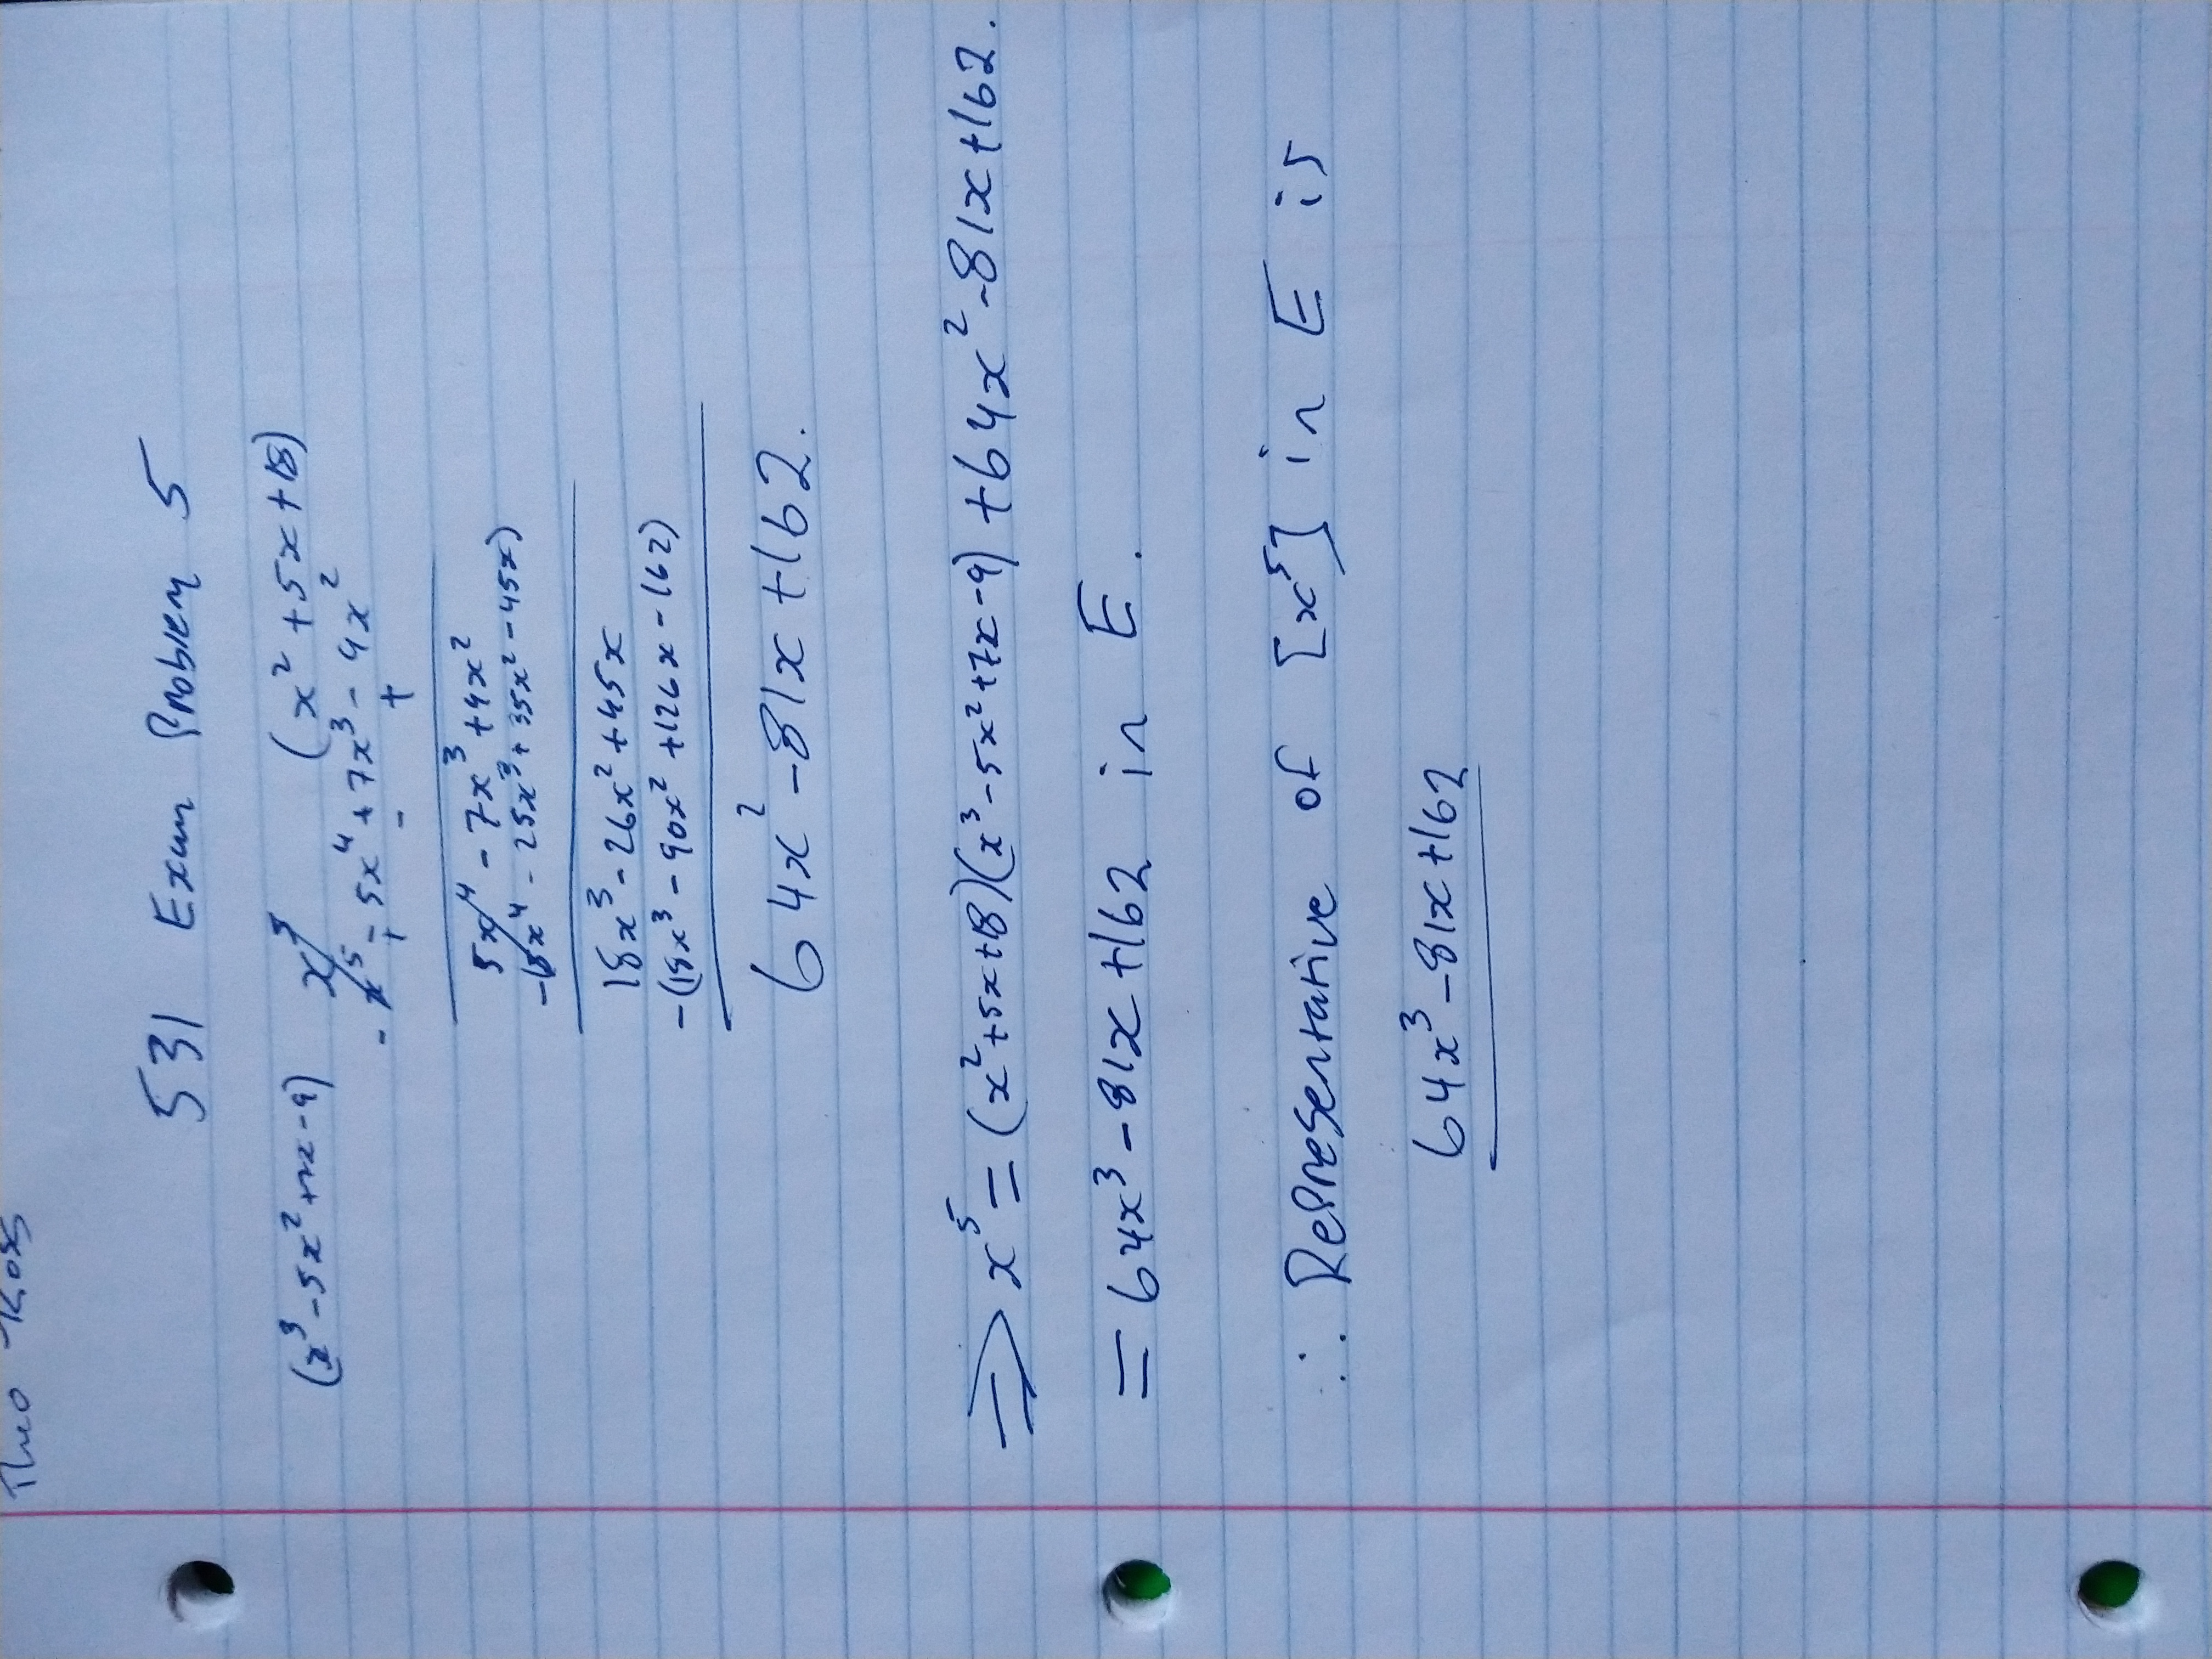
\includegraphics[angle=270,origin=c]{prob5.jpg}}
\section{Problem 6}Find polynomials $p(x),q(x)$ and an integer $p$ such that $q(x)|p(x)$ as elements of $\Z_p[x]$ but that $q(x)\centernot|p(x)$ as elements of $\R[x]$. $p,q$ will necessarily have integral coefficients.\begin{proof}
Consider the polynomials $p(x)=x^2+1$, $q(x)=x+1$, and $p=2$. Since in $\Z_2[x]$, $-x=x$, we can divide $x^2+1$ by $(x+1)$ leaving $(x+1)$. $$(x+1)(x+1)=x^2+2x+1\equiv x^2+1\in\Z_2[x]$$ Therefore, in $\Z_2[x]$, $q(x)|p(x)$. Now consider these two polynomials in $\R[x]$. Again trying to do long division, we end with a remainder of 2, and therefore $q(x)\centernot|p(x)$.
\end{proof}
\end{document}
